\documentclass[UTF8]{ctexart}

\usepackage{anyfontsize}
\usepackage{geometry}
    \geometry{left=4cm,right=4cm,top=2cm,bottom=2cm}
\usepackage{amsmath, amssymb, amsthm}
    \newtheorem{definition}{定义}
    \newtheorem{theorem}{定理}
    \newtheorem*{example}{例}
\usepackage{caption} 	 % 标题
\usepackage{xcolor} 	 % 颜色
\usepackage{graphicx} 	 % 引用图片
\usepackage{float}
\usepackage{framed} 	 % 方框 \begin{framed}
\usepackage{indentfirst} 	 % 首行缩进 
    \setlength{\parindent}{0em}
\usepackage{setspace} 	 % 行间距 \begin{spacing}{arg}
\usepackage{extarrows} 	 % 箭头宏包 \xLongrightarrow 
\usepackage{esvect} 	 % 向量箭头 \vv{}
\usepackage{siunitx} 	 % 国际单位 \si{unit} \SI{number}{unit} 
\usepackage{esint} 	 % 积分符号
\usepackage{mathrsfs}

% font
\newcommand{\ve}[1]{\boldsymbol{\mathbf{#1}}}
\newcommand{\unit}[1]{\boldsymbol{\mathbf{\hat{#1}}}}
\newcommand{\mcal}{\mathcal}
\newcommand{\mscr}{\mathscr}
% common symbol
\newcommand{\E}{\mathrm e}
\renewcommand{\I}{\mathrm i}
\newcommand{\R}{\mathbb R}
\newcommand{\Z}{\mathbb Z}
\newcommand{\N}{\mathbb N}
\newcommand{\Q}{\mathbb Q}
\newcommand{\C}{\mathbb C}
% differentiation
\def \DD #1.#2.#3 {\dfrac{d^{#1} #2}{d #3^{#1}}}
\def \PP #1.#2.#3 {\dfrac{\partial^{#1} #2}{\partial #3^{#1}}}
\def \dd #1.#2 {\dfrac{d #1}{d #2}}
\def \pp #1.#2 {\dfrac{\partial #1}{\partial #2}} 
\newcommand{\del}{\nabla}
% matrix
\newcommand{\transp}{^{\top}}
\DeclareMathOperator{\tr}{tr}

\pagestyle{empty}

\begin{document}
\section{微分形式初步}
注: 本文中向量使用圆括号或尖括号表示, 如: $ (x, y) $ 和 $ \left\langle 2, 3 \right\rangle $.
\subsection{微分}
\begin{definition}[\textbf{微分}]
    对于一元函数 $ y = f(x) $ 定义域中一点 $ x $, 有 $ \Delta y = f(x_0 + \Delta x) - f(x_0) = A \Delta x + o(\Delta x) $, 其中 $ A $ 是不依赖于 $ \Delta x $ 的常数, 则称 $ f $ 在 $ x_0 $ 可微. 并记 $ f $ 的微分等于其线性主部: \[ df(x_0) = A \Delta x  .\]
\end{definition}
\begin{theorem}[\textbf{微分与导数}]
    若 $ f $ 在 $ x_0 $ 可导, 则 $ f $ 在 $ x_0 $ 处可微, 则 $ df(x_0) = f'(x_0) \Delta x = f'(x_0) \,dx $. 若 $ f $ 在定义域内每一点均可微, 则 $ df = f'(x) \,dx $.
\end{theorem}

微分可推广到多元函数和向量函数上:
\begin{definition}[\textbf{多元函数微分}]
    设 $ f(x_1, \dots, x_n) \colon \R^n \to \R $, 则 \[ df = f_{x_1} \,dx_1 + \cdots + f_{x_n} \,dx_n = \sum_{i = 1}^{n} \pp {f}.{x_i} \,dx_i .\]

    设向量函数 $ \ve F = \langle F_1, F_2, \dots, F_n \rangle $, 其中每个分量 $ F_i $ 均同为一元或多元标量函数, 则 \[ d\ve F = \langle dF_1, dF_2, \dots, dF_n \rangle .\]
\end{definition}
上面内容阐述了: 对向量(函数)求导/微分, 即是对其分量分别求导/微分.

\begin{example}
    $ \ve F(x) = \langle x, x^2, x^3 \rangle $, 则 $ d\langle x, x^2, x^3 \rangle = \langle dx, d(x^2), d(x^3) \rangle = \langle dx, 2x\,dx, 3x^2\,dx \rangle $

    $ \ve F(x, y) = \langle xy, x + y \rangle $, 则 $ d\langle xy^2, x + y \rangle = \langle d(xy^2), d(x + y) \rangle = \langle y^2\,dx + 2xy\,dy, dx + dy \rangle $
\end{example}

同样, 对向量函数求导原理相同, 也有:
\vskip 0.5em
$ \ve F(x) = \langle x, x^2, x^3 \rangle $, 则 $ \dd {\ve F(x)}.{x} = \left\langle (x)', (x^2)', (x^3)' \right\rangle = \left\langle x, 2x, 3x^2 \right\rangle $
\vskip 1em

事实上, 对一个标量函数 $ f $ 微分, 得到的 $\displaystyle    f' \,dx $ 便是微分形式. 而积分 $\displaystyle \int f\,dx $, 重积分 $\displaystyle \iint_D f \,dx \,dy $, 标量场/向量场中的曲线/曲面积分中, 积分的对象也是微分形式.

\subsection{微分形式定义}
以二元函数 $ f(x, y) = \cos x^2 + \sin y^2 $ 为例, 求其微分:
\[ df = f_x \,dx + f_y \,dy = -2 x\sin x^2 \,{\color{red} dx} + 2 y \cos y^2 \,{\color{red} dy} .\]

上面出现的 $ dx $, $ dy $ 就是最简单的微分形式.

\begin{definition}[\bf 微分形式]
    把 $ \R^n $ 中的 $ dx_1 $, $ dx_2 $, $ \dots $, $ dx_n $ 叫做\textbf{基本$1$-形式}.
\end{definition}

同时, 在其上定义一种乘法运算 --- \textbf{楔积}, 让其满足反交换律:
\[ dx_i \land dx_j = -\, dx_j \land dx_i .\]

像这样, 两个基本$ 1 $-形式的楔积 $ dx_i \land dx_j $ 被称为基本$ 2 $-形式. 类似地, 还有基本$ 3 $-形式: \[ dx_i \land dx_j \land dx_k .\]

一个函数与基本$ k $-微分形式相乘就得到单项式$ k $-形式, 如:
\[ {\color{red} 3}\, {\color{blue} dx} \qquad (\text{单项式} 1\text{-形式}) \]
\[ {\color{red} 2xy} \,{\color{blue} dx \land dy} \qquad (\text{单项式}2\text{-形式}) \]
\[ {\color{red} (x - z)} \,{\color{blue} dx \land dz \land dy} \qquad (\text{单项式}3\text{-形式}) \]

函数定义为次数为 $ 0 $ 的微分形式.
\vskip 1em

多个单项式$ k $-形式相加就得到$ k $-形式, 如:
\[ {\color{blue} dx} + 2 x\,{\color{blue} dy} - xyz \,{\color{blue} dz} \qquad(\text{$ 1 $-形式}) \]
\[ - {\color{blue} dx \land dy} + x y \,{\color{blue} dy \land dz} - yz^2/x \,{\color{blue}dz \land dx} \qquad(\text{$ 2 $-形式}) \]

将楔积看作一种乘法, 微分形式的次数就好比是关于基本$ 1 $-形式 $ dx_i $ 的多项式的次数.

\subsubsection{楔积}
楔积 $ \land $ 满足如下性质:
\begin{enumerate}
    \item 反交换律: $ \omega_1 $, $ \omega_2 $ 分别为 $ k $-, $ l $-形式 \[ \omega_2 \land \omega_1 = (-1)^{k l}\, \omega_2 \land \omega_1 \]
    \item 分配律: \[ \omega \land (f + g) = \omega \land f + \omega \land g \]\[ (f + g) \land \omega = f \land \omega + g \land \omega \]
    \item 结合律: \[ \omega_1 + (\omega_2 + \omega_3) = (\omega_1 + \omega_2) + \omega_3 \]
\end{enumerate}

推论: \[ \omega \land \omega = 0 \]\[ dx_i \land dx_j = -\, dx_j \land dx_i \]




\newpage
\section{微分形式的微分}
设 $ \omega $ 是一个 $ k $-形式, 定义对其的微分运算 $ d\omega $, 微分后产生一个 $ (k + 1) $-形式, 这一运算也称外微分. 现有微分形式 $ \omega $ 和 $ \eta $, 外微分 $ d $ 满足:
\begin{enumerate}
    \item 若 $ f $ 为函数(即 $ 0 $-形式), $ df $ 就是 $ f $ 的微分
    \item 线性: \[ d(\omega_1 \pm \omega_2) = d\omega_1 \pm d\omega_2 \]\[ d(C \omega) = C\, d\omega \quad, (C \text{ 为常数}) \]
    \item \[ d(d\omega) = 0 \] \vskip -1em
    \item 乘法($ \omega $ 的次数为 $ \deg \omega $): \[ d(\omega \land \eta) = d\omega \land \eta + (-1)^{\deg \omega} \omega \land d\eta \]
\end{enumerate}

\begin{example}
    对于单项式$ k $-微分形式 $ f \omega = f\,dx_1\land \cdots \land dx_k $, 其中 $ f $ 为函数:
    \begin{align*}
        d(f \omega) = d(f \land \omega) &= df \land \omega + (-1)^{0} f \land d\omega \\
        &= df \land \omega + f \land d\omega \\
        &= df \land \omega + f \land d(dx_1 + \cdots + dx_k) \\
    \end{align*}
    \vskip -2em
    由归纳法可以证明: $ d(dx_1 + \cdots + dx_k) = 0 $, 所以单项式$ k $-形式的微分:
    \[ d(f \land dx_1 \land \cdots dx_k) = df \land dx_1 \land \cdots dx_k \] 

    此时再通过一元函数微分或全微分公式, 将 $ df $ 展开, 利用楔积的性质化简.
\end{example}

根据外微分的线性性质, 对任意 $ k $-形式微分, 总可以拆分为几个单项式 $ k $-形式的微分, 而单项式形式的微分由上面的例子很容易求得.

\begin{example}
    对于二元函数 $ P(x, y) $, $ Q(x, y) $. 计算 $ d(P \,dx + Q \,dy ) $:

    \[ d(P \,dx + Q \,dy ) = d(P \,dx) + d(Q \,dy) = dP \land dx + dQ \land dy \]
    
    由全微分公式:
    \begin{align*}
        dP \land dx + dQ \land dy &= (P_x \,dx + P_y \,dy) \land dx + (Q_x \,dx + Q_y \,dy) \land dy \\
        &= P_x \,dx \land dx + P_y \,dy \land dx + Q_x \,dx \land dy + Q_y \,dy \land dy \\
        &= P_y\, dy \land dx + Q_x \,dx \land dy \\
        &= -P_y\, dx \land dy + Q_x \,dx \land dy \\
        &= \left( \pp {Q}.{x} - \pp {P}.{y} \right) \,dx \land dy.
    \end{align*}
\end{example}




\section{微分形式的应用}
在曲线/曲面积分中, 微分$ 1 $-形式 $ dx $, $ dy $, $ dz $ 被理解为\textbf{有向长度}. $ 2 $-形式 $ dx \land dy $, $ dy \land dz $, $ dz \land dx $ 被理解为\textbf{有向面积}.
\vskip 1em

在二重积分
\[ \iint_D f(x, y) \,dx\,dy \]
中, 我们定义 $ Oxy $ 平面上方的体积为正, 平面下方的体积为负. 在一元函数定积分中也有相似定义. 这里就已经出现定向的概念, 我们把 $ XY $ 平面上方定为正向, 下方定位负向, 所以才有二重积分中体积正负的定义.
\vskip 1em

类比叉乘的定义, $ dx $, $ dy $ 看作是 $ x $ 轴, $ y $ 轴正向的向量, $ dx \land dy $ 得到的向量垂直于 $ dx $, $ dy $ 张成的平面(方向 $ z $ 轴正向). 因此我们将 $ dx \land dy $ 即 $ z $ 轴正向作为投影正负的判断. 例如, 对于 $ dx \land dy $, 取曲面上侧为正向, 则将曲面投影至 $ Oxy $ 平面后, 法向量朝上, 与 $ dx \land dy $ 方向相同, 所以投影面积为正; 取曲面下侧为正向, 投影后, 法向量朝下, 与 $ dx \land dy $ 方向相反, 所以投影面积为负. 由此可以将二重积分写成
\[ \iint_D f \,dx\,dy = \iint_D f \,dx \land dy \]

如果写成 $ dy \land dx $, 则表示 $ XY $ 上方体积为负, 下方体积为正:
\[ \iint_D f \,dy \land dx = - \iint_D f \,dx\,dy \]


\subsection{计算向量场中的曲面积分}
设向量场 $ \ve F = (P, Q, R) $, 可定向曲面 $ \ve S $. 计算 $\displaystyle \iint_{\ve S} \ve F \cdot d\ve S $:
\vskip 1em

已知面积向量 $ d\ve S = (dy \land dz, dz \land dx, dx \land dy) $, 改写曲面积分形式:
\[ I = \iint_{\ve S} \ve F \cdot d\ve S = \iint_{\ve S} P \,dy \land dz + Q \,dz \land dx + R \,dx \land dy ,\]

此时, $ x $, $ y $, $ z $ 轴正向为投影面积的正向. 将 $ x, y, z $ 参数化, 此处以 $ \big(x, y, z(x, y)\big) $ 为例, 由全微分及楔积的性质:
\begin{align*}
    I &= \pm \iint_{\ve S} P \,dy \land (z_x\,dx + z_y\,dy) + Q \,(z_x\,dx + z_y\,dy) \land dx + R \,dx \land dy \\
    &= \pm \iint_{D_{xy}} P z_x \,dy \land dx + Q z_y \,dy \land dx + R \,dx \land dy \\
    &= \pm \iint_{D_{xy}} (- P z_x - Q z_y + R) \,dx \land dy \\
    &= \pm \iint_{D_{xy}} (- P z_x - Q z_y + R) \,dx\,dy
\end{align*}
注意: $ dx \land dy $ 和前面的正负号 $ \pm $ 说明, 若曲面在 $ Oxy $ 面投影为正(法向量朝 $ z $ 轴正向), 则积分取正; 投影为负(法向量朝 $ z $ 轴负向), 则积分计算完毕后还要取负.  


\subsection{格林/高斯/斯托克斯公式的统一}
由第二节, 当 $ \omega = P \,dx + Q\, dy $ 时:
\[ d\omega = \left( \pp {Q}.{x} - \pp {P}.{y} \right) \,dx \land dy .\]

同理可以算得, 当 $ \omega = P \,dy \land dz + Q \,dz \land dx + R \,dx \land dy $ 时:
\[ d\omega = \left( \pp {P}.{x} + \pp {Q}.{y} + \pp {R}.{z} \right) dx \land dy \land dz .\]

当 $ \omega = P \,dx + Q \,dy + R \,dz $ 时:
\[ d\omega = \begin{vmatrix}
    dy \land dz & dz \land dx & dx \land dy \\[0.5em]
    \pp {}.{x} & \pp {}.{y} & \pp {}.{z} \\[0.7em]
    P & Q & R
\end{vmatrix} .\]

所以三个公式可以统一为:
\[ \int_{\partial M} \omega = \int_{M} d\omega .\]

其中, $ \partial M $ 表示区域 $ M $ 的边界.


\subsection{路径无关}
\begin{theorem}[\bf 梯度定理]
    $ f $ 是一个多元标量函数, $ \gamma[\ve p, \ve q] $ 是一段曲线, 位置向量 $ \ve p $, $ \ve q $ 分别指向起点和终点:
    \[ f(\ve q) - f(\ve p) = \int_{\gamma} \del f(\ve r) \cdot d\ve r .\]
\end{theorem}

这一定理说明了, 如果向量场 $ \ve F $ 为(某一标量场的)梯度场, 即: $ \ve F = \del G $, 则这个向量场中的曲线积分是路径无关的, 等于终点 $ \ve b $, 起点 $ \ve a $ 处的原函数函数值之差:
\[ \int_{\ve a}^{\ve b} \ve F \cdot d \ve r = G(\ve b) - G(\ve a) \]

一个场是路径无关的, 则也称其为保守场.
\vskip 1em

\begin{theorem}
    曲线积分 $\displaystyle \int_{\ve C} P \,dx + Q \,dy $ 与路径无关的的充分必要条件是:
    \[ \pp {P}.{y} = \pp {Q}.{x} .\]
\end{theorem}


\subsection{全微分形式}
若 $ \R^2 $ 中的 $ P \,dx + Q \,dy $ 能写成某个二元函数的全微分, 则称 $ P \,dx + Q \,dy $ 是完全的. 
\vskip 0.5em
那么给定一个 $ P \,dx + Q \,dy $ 如何判断是否存在对应的 $ f $ 使得 $ df = P\,dx + Q \,dy $ 呢?

\begin{theorem}
    若函数 $ P(x, y) $ 和 $ Q(x, y) $ 在 $ D $ 内具有一阶连续偏导数, 则 $ P\,dx + Q\,dy $ 在 $ D $ 内能写成 $ f(x, y) $ 全微分的充分必要条件为:
    \[ \pp {P}.{y} = \pp {Q}.{x} .\]
\end{theorem}

如果 $ P_y = Q_x $, 则 $ P\,dx + Q\,dy $ 能写成全微分形式, 于是曲线积分
\[ \int_{\ve a}^{\ve b} P\,dx + Q\,dy = \int_{\ve a}^{\ve b} \pp {f}.{x} \,dx + \pp {f}.{y} \,dy = \int_{\ve a}^{\ve b} df = f(\ve b) - f(\ve a) .\]

这与上一个定理($ P_y = Q_x \Leftrightarrow \text{路径无关} $ )对应.
\vskip 1em

如何寻找对应的 $ df = P\,dx + Q\,dy $? 既然能写成全微分形式, 则 $ P_y = Q_x $, 所以 $\displaystyle \int_{\ve C} P\,x + Q\,dy $ 是路径无关的, 其积分值就等于 $ f $ 在终点处的值减去起点处的值. 故取任意一个起点 $ (x_0, y_0) $, 求此处到 $ (x, y) $ 的任意路径积分
\[ \int_{(x_0, y_0)}^{(x, y)} P\,dx + Q\,dy = f(x, y) - f(x_0, y_0) ,\]

即找到了 $ f(x, y) $. 通常为计算方便, 取水平和竖直的折线路径 $ (x_0, y_0) \to (x, y_0) \to (x, y) $, 此时:
\begin{align*}
    \int_{(x_0, y_0)}^{(x, y)} P\,dx + Q\,dy &= \int_{x_0}^x P(u, y_0) \,du + \int_{y_0}^y Q(x, v) \,dv \qquad(\text{先 $ x $ 后 $ y $}) \\
    &= \int_{y_0}^{y} Q(x_0, v) \,dv + \int_{x_0}^{x} P(u, y) \, du. \qquad(\text{先 $ y $ 后 $ x $})
\end{align*}




总结一下, 对于 $\displaystyle \int_{\ve C} \ve F \cdot d\ve r = \int_{\ve C} P\,dx + Q\,dy $:
\vskip 1em
\begin{figure}[H]
    \centering
    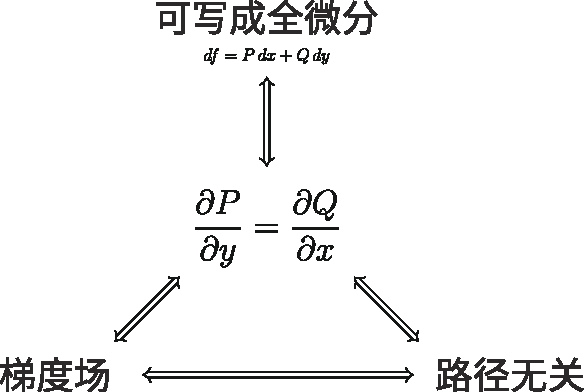
\includegraphics[width = 0.5\linewidth]{untitled1.pdf}
\end{figure}

以上四种命题均可任意互相推导.




\end{document}